\section{非线性参数的拟合}
\label{sec:opt-fit-nonlinear}

把函数写成$\sum_jw_j\varphi_j$时，读数对参数是线性的。指数衰减$\theta_1e^{-\theta_2t}$、带可学习位置的核函数、神经网络等模型则不然：候选$f_{\bm\theta}$对参数$\bm\theta\in\mathbb R^d$非线性，残差不再是$\bm\theta$的仿射函数。本节的思路是在当前点把残差或模型输出线性化，借用上一节的最小二乘机器求出候选步，再回到原目标判断这一步能不能接受。线性化只在当前点附近可信，这一点贯穿三种方法：Gauss--Newton法直接相信线性模型，Levenberg--Marquardt法用阻尼控制走出多远，广义Gauss--Newton法把同样的做法推广到一般损失。

\subsection{残差线性化与Gauss--Newton法}
\label{sec:opt-fit-gauss-newton}

\paragraph{梯度、Hessian与被省略的项}
设残差$\bm r(\bm\theta)=(r_1(\bm\theta),\dots,r_n(\bm\theta))^\top$二次连续可微，$\bm J(\bm\theta)\in\mathbb R^{n\times d}$是它的Jacobian矩阵，$\bm J_{i,:}=\nabla r_i(\bm\theta)^\top$。非线性最小二乘目标$F(\bm\theta)=\tfrac12\|\bm r(\bm\theta)\|_2^2$的梯度与Hessian由链式法则得到：
\begin{equation}
  \nabla F=\bm J^\top\bm r,\qquad
  \nabla^2F=\bm J^\top\bm J+\sum_{i=1}^nr_i\nabla^2r_i .
  \label{eq:opt-fit-nls-derivatives}
\end{equation}
第二项是各残差的二阶导数按残差大小加权求和。在当前点$\bm\theta$把残差线性化，$\bm r(\bm\theta+\bm p)\approx\bm r+\bm J\bm p$，代入目标得到线性最小二乘子问题
\begin{equation}
  \min_{\bm p\in\mathbb R^d}\ m(\bm p)=\frac12\|\bm r+\bm J\bm p\|_2^2 .
  \label{eq:opt-fit-gn-model}
\end{equation}
$m$的Hessian是$\bm J^\top\bm J$，所以\term{Gauss--Newton法}（Gauss--Newton method）相当于在牛顿法中省略式~\eqref{eq:opt-fit-nls-derivatives}的第二项。当残差小或残差近似线性时，被省略的项小，$\bm J^\top\bm J$是$\nabla^2F$的良好近似，而且它总是半正定的，计算时只需要一阶导数。

\paragraph{求步：用最小二乘而不是正规方程}
子问题~\eqref{eq:opt-fit-gn-model}的正规方程是$\bm J^\top\bm J\bm p=-\bm J^\top\bm r$，但应直接对$\bm J$做QR或奇异值分解来解。原因在于条件数：$\kappa(\bm J^\top\bm J)=\kappa(\bm J)^2$。若$\bm J$的两个奇异值为$1$与$10^{-4}$，$\kappa(\bm J)=10^4$，而正规方程的条件数为$10^8$；在双精度下，后者可能丢失约八位有效数字，前者只丢失约四位。

\paragraph{秩亏时取最小范数步并检验下降}
$\bm J$满列秩时，子问题有唯一解$\bm p=-\bm J^\dagger\bm r$。秩亏时子问题有一族解，相差$\ker\bm J$中的向量；沿这些方向线性模型不变，却不说明原目标不变。通常取其中欧氏范数最小的一个，仍记为$\bm p=-\bm J^\dagger\bm r$。这个方向是不是原目标的下降方向？直接计算方向导数：
\[
  \langle\nabla F,\bm p\rangle=-\bm r^\top\bm J\bm J^\dagger\bm r=-\|\bm J\bm J^\dagger\bm r\|_2^2 ,
\]
这里用了$\bm J\bm J^\dagger$是到$\operatorname{range}\bm J$的正交投影。由于$\operatorname{range}\bm J$与$\ker\bm J^\top$正交互补，$\bm J\bm J^\dagger\bm r=\bm 0$当且仅当$\bm J^\top\bm r=\nabla F=\bm 0$。所以只要当前点不是驻点，Gauss--Newton方向就是下降方向。下降方向只保证足够小的步长使$F$下降，单位步长未必如此，所以实际实现用原目标$F$做回溯线搜索，接受满足充分下降条件的步长；回溯规则见第~\ref{chap:opt-smooth}章。

\paragraph{局部二次收敛的条件}
在解$\bm\theta^\star$附近，若残差为零（$\bm r(\bm\theta^\star)=\bm 0$）、$\bm J(\bm\theta^\star)$满列秩、$\bm J$在$\bm\theta^\star$附近Lipschitz连续，则从足够近的初值出发、取单位步长的Gauss--Newton迭代二次收敛到$\bm\theta^\star$\scite{math-nocedal2006numerical}。一维例子可以完整验算：$r(\theta)=\theta^2-4$，零残差解$\theta^\star=2$，$J=2\theta$，Gauss--Newton步给出
\[
  \theta^+=\theta-\frac{\theta^2-4}{2\theta}=\frac{\theta^2+4}{2\theta},\qquad
  \theta^+-2=\frac{(\theta-2)^2}{2\theta}.
\]
从$\theta=3$出发，误差依次为$1$、$1/6$、$1/156\approx6.4\times10^{-3}$、约$1.0\times10^{-5}$，每步误差约为上一步的平方。

\paragraph{非零残差时被省略的项决定收敛}
残差在解处不为零时，被省略的$\bm S=\sum_ir_i\nabla^2r_i$不再消失。设$\bm\theta^\star$满足$\nabla F(\bm\theta^\star)=\bm J^\top\bm r=\bm 0$且$\bm J^\star=\bm J(\bm\theta^\star)$满列秩，把单位步长的迭代看成映射$\bm\theta\mapsto\bm\theta-(\bm J^\top\bm J)^{-1}\bm J^\top\bm r$。在$\bm\theta^\star$处求导，由于$\bm J^\top\bm r=\bm 0$，对$(\bm J^\top\bm J)^{-1}$求导的那一项消失，剩下
\[
  \bm I-(\bm J^{\star\top}\bm J^\star)^{-1}\bigl(\bm J^{\star\top}\bm J^\star+\bm S^\star\bigr)=-(\bm J^{\star\top}\bm J^\star)^{-1}\bm S^\star .
\]
这个矩阵的谱半径小于$1$时迭代在$\bm\theta^\star$附近线性收敛，速率由它决定；谱半径大于$1$时$\bm\theta^\star$对单位步长迭代是排斥的。所以残差大、残差曲率大时，Gauss--Newton可能很慢甚至不收敛。还有两种情形会破坏局部模型：$\bm J$的秩在迭代中变化，使最小范数步突然变长；子问题只被粗略求解，使所得的步连线性模型都没有充分下降。线性模型下降不能直接当作原目标下降，这正是下一小节要处理的问题。

\subsection{Levenberg--Marquardt法}
\label{sec:opt-fit-levenberg-marquardt}

\paragraph{加阻尼的子问题}
线性化只在当前点附近可信，步子越长，模型越可能失真。最简单的控制办法是惩罚步长本身，求
\begin{equation}
  \min_{\bm p}\ \frac12\|\bm r+\bm J\bm p\|_2^2+\frac\tau2\|\bm p\|_2^2,
  \qquad\text{即}\qquad
  (\bm J^\top\bm J+\tau\bm I)\bm p=-\bm J^\top\bm r ,
  \label{eq:opt-fit-lm-step}
\end{equation}
其中$\tau>0$是阻尼参数（本章用$\tau$，以免与正则化参数$\lambda$、核积分算子的特征值$\mu_j$混淆）。这就是\term{Levenberg--Marquardt法}（Levenberg--Marquardt method）的求步方程。$\tau>0$使系数矩阵正定，即使$\bm J$秩亏，步长也唯一。与第~\ref{sec:opt-fit-linear-basis}小节一样，它可以写成增广最小二乘$\min_{\bm p}\tfrac12\bigl\|\bigl[\begin{smallmatrix}\bm J\\\sqrt\tau\bm I\end{smallmatrix}\bigr]\bm p+\bigl[\begin{smallmatrix}\bm r\\\bm 0\end{smallmatrix}\bigr]\bigr\|_2^2$，用QR或LSQR求解；迭代求解时以线性系统的残差控制精度。

阻尼与正则化外形相似，作用不同。正则项$\tfrac\lambda2\|\bm\theta\|^2$永久改变目标及其最小点；阻尼$\tfrac\tau2\|\bm p\|^2$只惩罚本轮位移，在驻点处$\nabla F=\bm 0$使$\bm p=\bm 0$，不改变原目标的任何驻点。

\paragraph{阻尼在Gauss--Newton步与梯度方向之间插值}
用$\bm J$的奇异值分解$\bm J=\sum_k\sigma_k\bm u_k\bm v_k^\top$可以看清$\tau$的作用：
\[
  \bm p(\tau)=-\sum_k\frac{\sigma_k}{\sigma_k^2+\tau}(\bm u_k^\top\bm r)\bm v_k,\qquad
  \|\bm p(\tau)\|_2^2=\sum_k\frac{\sigma_k^2(\bm u_k^\top\bm r)^2}{(\sigma_k^2+\tau)^2}.
\]
由此读出三点。$\tau\downarrow0$时，系数趋于$1/\sigma_k$，$\bm p(\tau)\to-\bm J^\dagger\bm r$，即最小范数Gauss--Newton步。$\tau\to\infty$时，$\tau\bm p(\tau)\to-\sum_k\sigma_k(\bm u_k^\top\bm r)\bm v_k=-\bm J^\top\bm r=-\nabla F$，步子变短并转向负梯度方向。步长$\|\bm p(\tau)\|_2$随$\tau$单调递减。图~\ref{fig:opt-fit-lm-path}在一个两参数指数拟合问题上画出了整条路径$\bm\theta^{(0)}+\bm p(\tau)$：它从靠近最小点的Gauss--Newton点出发，随$\tau$增大缩回到起点附近，并在起点处与负梯度相切。大阻尼给出保守的梯度步，小阻尼给出大胆的模型步，$\tau$在两者之间连续调节。

\begin{figure}[!htbp]
  \centering
  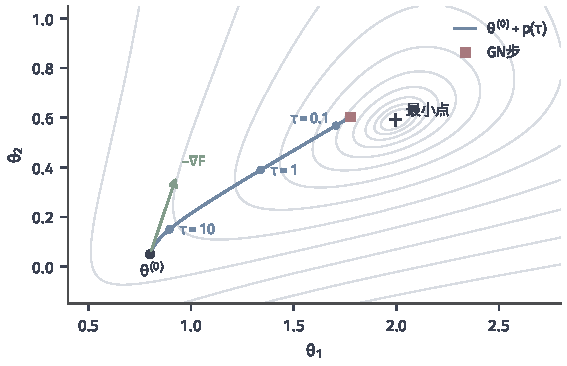
\includegraphics[width=96mm]{figures/03-optimization-evolution-and-signals/01-optimization/matplotlib/c8-lm-path/figure.pdf}
  \caption{Levenberg--Marquardt步随阻尼的变化。拟合模型$\theta_1e^{-\theta_2t}$到读数$t=0,\dots,4$，$y=(2.0,1.1,0.6,0.35,0.2)$；灰线为$\log_{10}F$的等值线，十字为最小点$(2.00,0.59)$。从$\bm\theta^{(0)}=(0.8,0.05)$出发，蓝线是$\tau$从$0$到$\infty$时的候选点$\bm\theta^{(0)}+\bm p(\tau)$，方块为$\tau=0$的Gauss--Newton点$(1.78,0.60)$，圆点标出$\tau=0.1,1,10$；绿色箭头为负梯度方向，大阻尼的步沿它离开起点。}
  \label{fig:opt-fit-lm-path}
\end{figure}

\paragraph{预报下降与接受检验}
候选步由模型算出，是否接受要回到原目标判断。用未加阻尼的线性模型$m(\bm p)=\tfrac12\|\bm r+\bm J\bm p\|_2^2$计算\term{预报下降}（predicted reduction）$\operatorname{pred}=m(\bm 0)-m(\bm p)$，与实际下降$\operatorname{ared}=F(\bm\theta)-F(\bm\theta+\bm p)$比较，比值
\begin{equation}
  \varrho=\frac{\operatorname{ared}}{\operatorname{pred}}
  \label{eq:opt-fit-lm-ratio}
\end{equation}
接近$1$说明模型可信，接近零或为负说明模型在这一步失真。式~\eqref{eq:opt-fit-lm-step}被精确求解时，预报下降总为正：由$\bm J^\top\bm r=-(\bm J^\top\bm J+\tau\bm I)\bm p$，
\[
  \operatorname{pred}=-\bm r^\top\bm J\bm p-\frac12\|\bm J\bm p\|_2^2
  =\bm p^\top(\bm J^\top\bm J+\tau\bm I)\bm p-\frac12\|\bm J\bm p\|_2^2
  =\frac12\|\bm J\bm p\|_2^2+\tau\|\bm p\|_2^2 ,
\]
它在$\bm p\ne\bm 0$（即$\nabla F\ne\bm 0$）时严格为正。因此若算出的预报下降不为正，应先检查求步是否足够精确或导数是否有误；若梯度已为零，则报告驻点并检查其性质。这里的比值检验与第~\ref{chap:opt-smooth}章信赖域方法的接受规则同源，阻尼$\tau$与信赖域半径扮演对偶的角色。

\begin{algorithm}[Levenberg--Marquardt法]
\label{alg:opt-fit-lm}
\begin{algorithmic}[1]
\Require 残差$\bm r$及其Jacobian、初值$\bm\theta^{(0)}$、初始阻尼$\tau^{(0)}>0$、接受阈值$0<\eta_a<\tfrac14$、梯度容许误差$\epsilon$
\Ensure 参数$\bm\theta$
\For{$t=0,1,2,\dots$}
  \State 计算$\bm r$、$\bm J$与$\nabla F=\bm J^\top\bm r$；若$\|\nabla F\|_2\le\epsilon$，返回$\bm\theta^{(t)}$
  \State 以增广最小二乘解式~\eqref{eq:opt-fit-lm-step}得$\bm p$，计算$\operatorname{pred}$与$\varrho$
  \If{$\varrho>\eta_a$}
    \State $\bm\theta^{(t+1)}\gets\bm\theta^{(t)}+\bm p$ \Comment{接受}
  \Else
    \State $\bm\theta^{(t+1)}\gets\bm\theta^{(t)}$ \Comment{拒绝}
  \EndIf
  \State 若$\varrho<\tfrac14$则$\tau^{(t+1)}\gets4\tau^{(t)}$；若$\varrho>\tfrac34$则$\tau^{(t+1)}\gets\tau^{(t)}/2$；否则不变
\EndFor
\end{algorithmic}
\end{algorithm}

每轮的主要代价是一次Jacobian计算与一次$(n+d)\times d$增广最小二乘求解；被拒绝的轮次只增大阻尼，不重新计算Jacobian。

\begin{example}[阻尼挽救一次发散的步]
\label{ex:opt-fit-lm-scalar}
取$r(\theta)=\theta^2-4$，$\theta^{(0)}=\tfrac12$，则$r=-\tfrac{15}4$，$J=1$，$F(\theta^{(0)})=\tfrac12\cdot\tfrac{225}{16}=\tfrac{225}{32}\approx7.03$。无阻尼时$p=-r/J=\tfrac{15}4$，新点$\theta=\tfrac{17}4$处$r=\tfrac{225}{16}$，$F=\tfrac{50625}{512}\approx98.9$，目标反而增大十几倍。取$\tau=4$，$p=-Jr/(J^2+\tau)=\tfrac{15/4}{5}=\tfrac34$，新点$\theta=\tfrac54$处$r=-\tfrac{39}{16}$，$F=\tfrac{1521}{512}\approx2.97$。预报下降为$\tfrac12(Jp)^2+\tau p^2=\tfrac9{32}+\tfrac{72}{32}=\tfrac{81}{32}$，实际下降为$\tfrac{225}{32}-\tfrac{1521}{512}=\tfrac{2079}{512}$，比值$\varrho=\tfrac{77}{48}\approx1.60>\tfrac34$，于是接受这一步，并把阻尼减半为$2$。
\end{example}

图~\ref{fig:opt-fit-gn-lm-scalar}把这个例子画了出来。黄色虚线是在$\theta^{(0)}$处线性化残差得到的模型$m$，它是一条开口向上、最小点远在$\theta=\tfrac{17}4$的抛物线，而原目标$F$在$\theta=2$之后迅速上升；Gauss--Newton步完全相信这条抛物线，跳过了真正的最小点。加阻尼后的模型（绿色点划线）在起点附近更陡地弯起，最小点被拉回到$\theta=\tfrac54$，这一步落在$F$确实下降的区域。阻尼控制的是线性化误差，而不只是让方程可逆：本例中$J=1$本来就可逆。

\begin{figure}[!htbp]
  \centering
  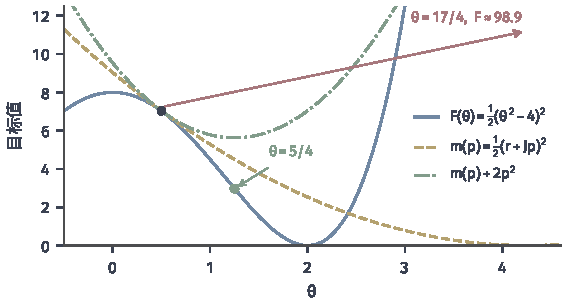
\includegraphics[width=96mm]{figures/03-optimization-evolution-and-signals/01-optimization/matplotlib/c8-gn-lm-scalar/figure.pdf}
  \caption{一维非线性最小二乘$F(\theta)=\tfrac12(\theta^2-4)^2$上的Gauss--Newton步与Levenberg--Marquardt步。蓝线为原目标，黑点为$\theta^{(0)}=\tfrac12$；黄色虚线为线性化模型$m(p)=\tfrac12(r+Jp)^2$，其最小点$\theta=\tfrac{17}4$处原目标约为$98.9$（红色箭头）；绿色点划线为加阻尼$\tau=4$的模型$m(p)+2p^2$，其最小点$\theta=\tfrac54$处原目标降到约$2.97$（绿点）。}
  \label{fig:opt-fit-gn-lm-scalar}
\end{figure}

\paragraph{条件与局限}
Levenberg--Marquardt法在每轮子问题上都有唯一解，配合比值检验能保证接受的步使原目标下降。但这不意味着找到全局最小点：非凸的$F$可能有多个局部最小点，算法停在哪一个取决于初值；收敛速率也没有统一的结论，在零残差且Jacobian满列秩的解附近，阻尼趋于零时它表现得像Gauss--Newton法，否则可能只有线性速率。若把它用作非线性残差IRLS的内层求解器，每轮要检查的是完整的加权代理~\eqref{eq:opt-fit-irls-surrogate}是否下降，而不只是检查一次线性化模型。

\subsection{一般损失与广义Gauss--Newton法}
\label{sec:opt-fit-ggn}

平方损失只是一种选择。分类模型常用交叉熵，稳健回归用Huber损失，模型的输出也可能是向量。本小节把Gauss--Newton的思路推广到一般损失：仍然把模型输出线性化，但对损失保留完整的二阶信息。

\paragraph{链式法则分出两类二阶项}
设第$i$个样本的模型输出为$\bm h_i(\bm\theta)\in\mathbb R^{q}$，损失为$\ell_i(\bm z)$，目标为$F(\bm\theta)=\frac1n\sum_{i=1}^n\ell_i(\bm h_i(\bm\theta))$。在当前点记输出Jacobian $\bm J_i=D\bm h_i(\bm\theta)\in\mathbb R^{q\times d}$、损失对输出的梯度$\bm a_i=\nabla\ell_i(\bm h_i)$与Hessian $\bm S_i=\nabla^2\ell_i(\bm h_i)$。链式法则给出
\[
  \nabla F=\frac1n\sum_i\bm J_i^\top\bm a_i,\qquad
  \nabla^2F=\frac1n\sum_i\Bigl[\bm J_i^\top\bm S_i\bm J_i+\sum_{k=1}^qa_{i,k}\nabla^2h_{i,k}\Bigr].
\]
第一项来自损失的曲率，第二项来自输出映射的曲率、按损失梯度加权。保留第一项、省略第二项，得到\term{广义Gauss--Newton矩阵}（generalized Gauss--Newton matrix）
\begin{equation}
  \bm H_{\mathrm{GN}}=\frac1n\sum_{i=1}^n\bm J_i^\top\bm S_i\bm J_i .
  \label{eq:opt-fit-ggn}
\end{equation}
平方损失$\ell_i(\bm z)=\tfrac12\|\bm z-\bm y_i\|_2^2$时$\bm S_i=\bm I$，它退回普通Gauss--Newton矩阵（相差因子$1/n$）。若每个$\ell_i$对输出凸且二次可微，则$\bm S_i\succeq\bm0$，从而$\bm H_{\mathrm{GN}}\succeq\bm0$。这只说明线性化后的模型是凸二次函数，复合目标$F$对参数仍可能非凸。

\paragraph{半正定不能认证没有负曲率}
一个标量例子说明两者的差距。取$n=1$，$h(\theta)=\theta^2$，$\ell(z)=\tfrac12(z-1)^2$，则$F(\theta)=\tfrac12(\theta^2-1)^2$。这里$J=2\theta$，$S=1$，$a=\theta^2-1$，$h''=2$，所以
\[
  \nabla^2F=4\theta^2+2(\theta^2-1)=6\theta^2-2,\qquad H_{\mathrm{GN}}=4\theta^2 .
\]
在$\theta=0.3$处，$H_{\mathrm{GN}}=0.36>0$，而真实曲率$\nabla^2F=-1.46<0$。广义Gauss--Newton矩阵总是半正定的，所以它不能用来认证一个驻点是局部最小点。输出映射是仿射函数时第二项为零，$\bm H_{\mathrm{GN}}=\nabla^2F$，这是舍项消失的充分条件；一般情形下，被舍去的项要另行估计。

\paragraph{矩阵自由求步}
参数很多时不能存储$d\times d$的$\bm H_{\mathrm{GN}}$，但可以计算它与任意向量$\bm v$的乘积：依次算输出方向导数$\bm J_i\bm v$、乘以损失曲率$\bm S_i(\bm J_i\bm v)$、再由反向传播得到$\bm J_i^\top(\bm S_i\bm J_i\bm v)$，对样本平均即得$\bm H_{\mathrm{GN}}\bm v$，代价约为两次前向与一次反向计算。求步方程
\[
  (\bm H_{\mathrm{GN}}+\tau\bm I)\bm p=-\nabla F
\]
在$\tau>0$与上述凸性条件下系数矩阵正定，可以用第~\ref{chap:opt-smooth}章的共轭梯度法（CG）求解，只调用矩阵向量积，并以相对残差控制内层精度。

从零初值出发的CG有一个有用的性质：每个中间近似解都是原目标的下降方向。记$\bm A=\bm H_{\mathrm{GN}}+\tau\bm I\succ\bm0$，$\bm g=\nabla F\ne\bm0$。CG的第$k$个近似$\bm p_k$在含$\bm g$的Krylov子空间中极小化$q(\bm p)=\tfrac12\bm p^\top\bm A\bm p+\bm g^\top\bm p$，于是$q(\bm p_k)\le q(-\alpha\bm g)<0$对足够小的$\alpha>0$成立，从而$\bm g^\top\bm p_k<-\tfrac12\bm p_k^\top\bm A\bm p_k<0$。因此即使提前停止CG，所得方向也能下降。接受与否仍用原目标判断：用真梯度检查$\langle\nabla F,\bm p\rangle<0$，再沿$\bm p$回溯，或像Levenberg--Marquardt法那样计算比值并调节$\tau$。
